\mysubsubsection{The Importance of Personal Touch}
We found personal contact to be an important factor in the process of finding a group to join. Forty-four percent of respondents reported that they first heard about the project they eventually joined through human contact, and 40\% cited a physical meeting or personal email exchange as the means taken to initially communicate with their project about the possibility of contribution. It is possible that this communication pattern may be biased by the unique academic setting that all respondents were in, as part of a course that facilitated in-person discussion about possible projects to join. Several respondents ended up participating in projects that other classmates were heavily involved in. Further research is needed to investigate whether most contributors to open collaboration projects have some personal connection with the project, or if the present results are unique to our specific situation.


\begin{figure}[ht!]
\centering
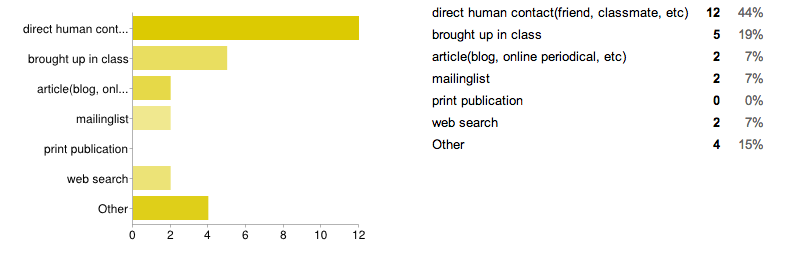
\includegraphics[width=120mm]{chapters/img/importance_of_personal_touch.png}
\caption{Importance of personal touch}
\label{overflow}
\end{figure}


Personal contact was also an important outreach method for 46\% of the projects surveyed, and we further examined whether this finding was related to the size of the group. An open-ended survey question about project outreach was qualitatively coded for personal contact, with responses which indicated efforts such as small in-person meetings and/or project member attendance and outreach at hackathons, workshops, conferences, and other community events that were not only held online. We did not find a dependence between group size and outreach through personal contact (Fisher’s Exact Test, p = 0.55). This finding suggests that both large and small groups rely on various types of in-person outreach to recruit new contributors. Since these organized group meetings are a common first contact point for many potential contributors, further research is needed to identify how different types and approaches to personal modes of outreach impact the recruitment of individuals with specific skills or motivations.


Most of the classmates report back that they have had physical contact to at least one of the projects contributors. This can have been through a talk at the university, through other classmates or through work. They report back that this was the initial trigger that made them know about the project by at the same time breaking down entry barriers since it was easier to get information when needed. Therefore many of the project are somehow connected to the Bay Area, which might be surprising as open source project often are seen as international where physical space plays a secondary role.